\thispagestyle{lichsutoanhocnone}
\pagestyle{lichsutoanhoc}
\graphicspath{{../lichsutoanhoc/pic/}}
\everymath{\color{lichsutoanhoc}}
\blfootnote{$^1$\color{lichsutoanhoc}Hà Nội.}
\begingroup
\AddToShipoutPicture*{\put(0,616){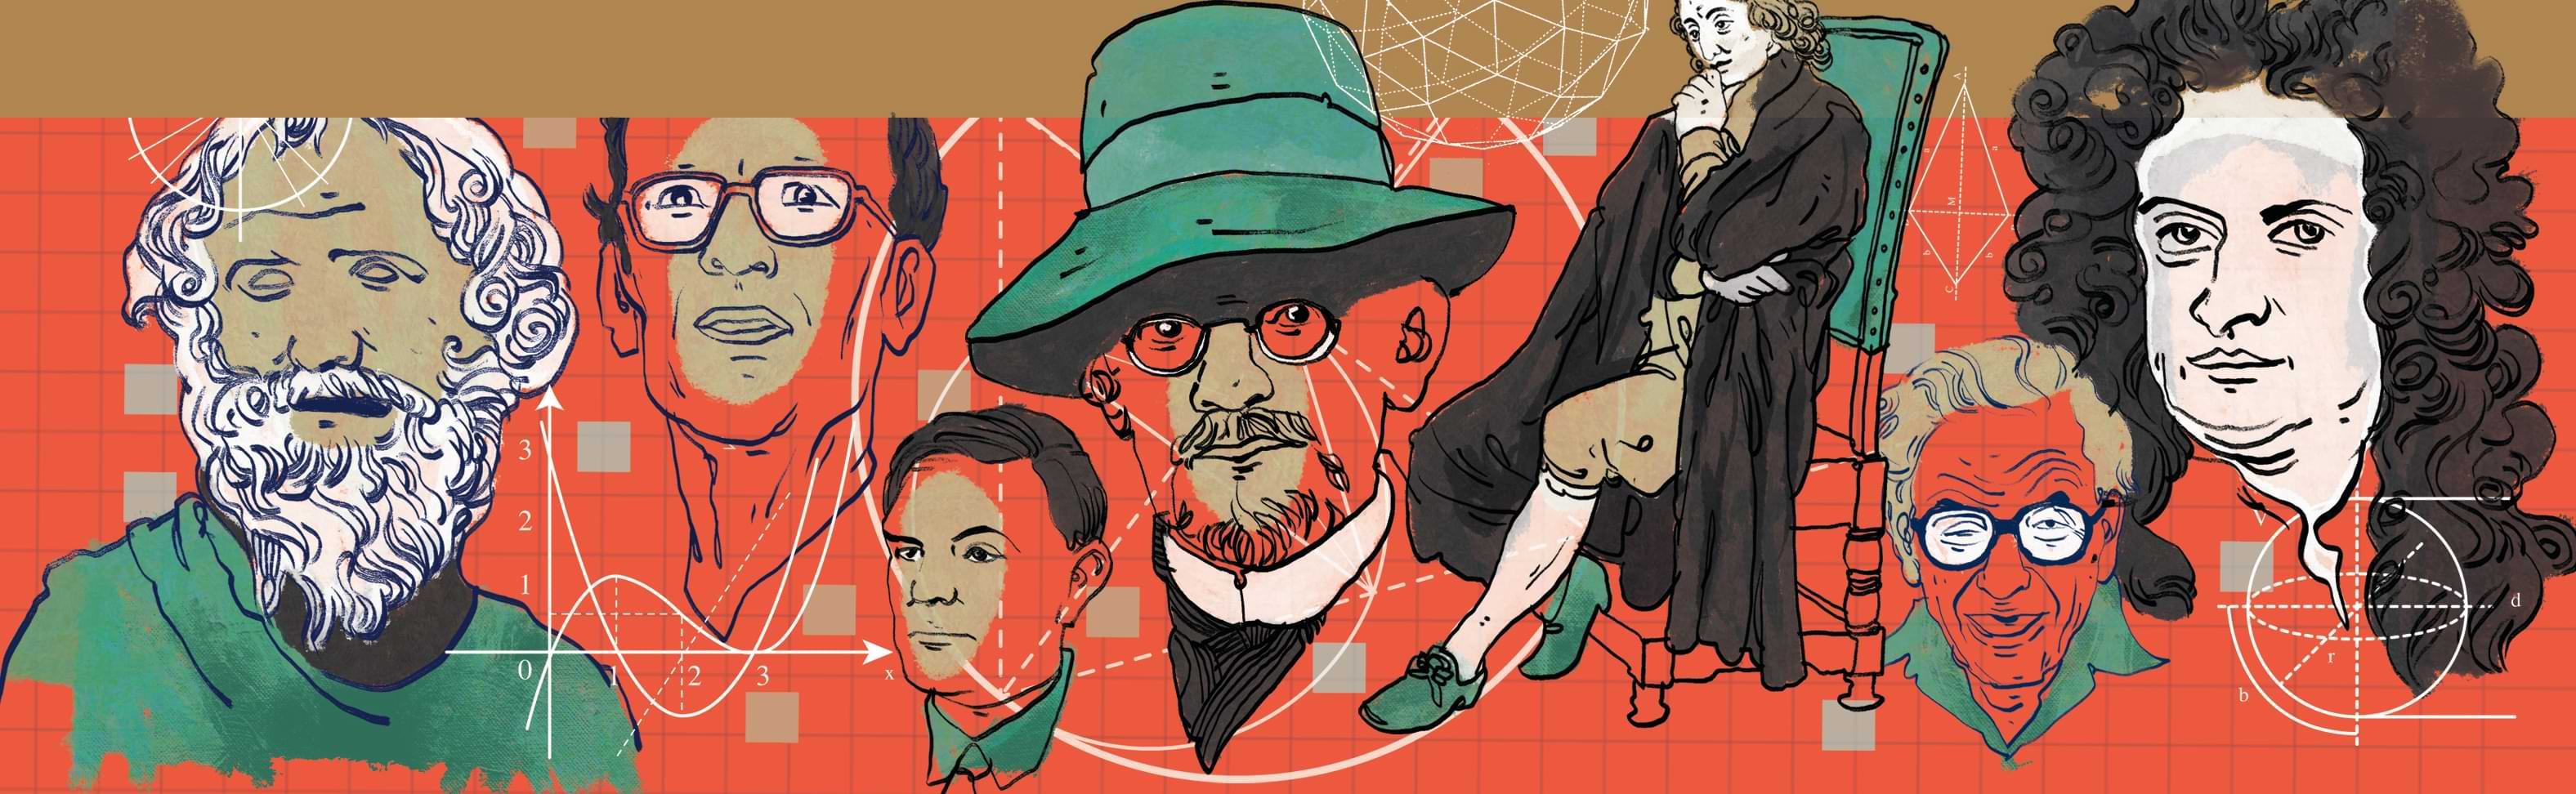
\includegraphics[width=19.3cm]{../bannerlichsu}}}
\AddToShipoutPicture*{\put(132,525){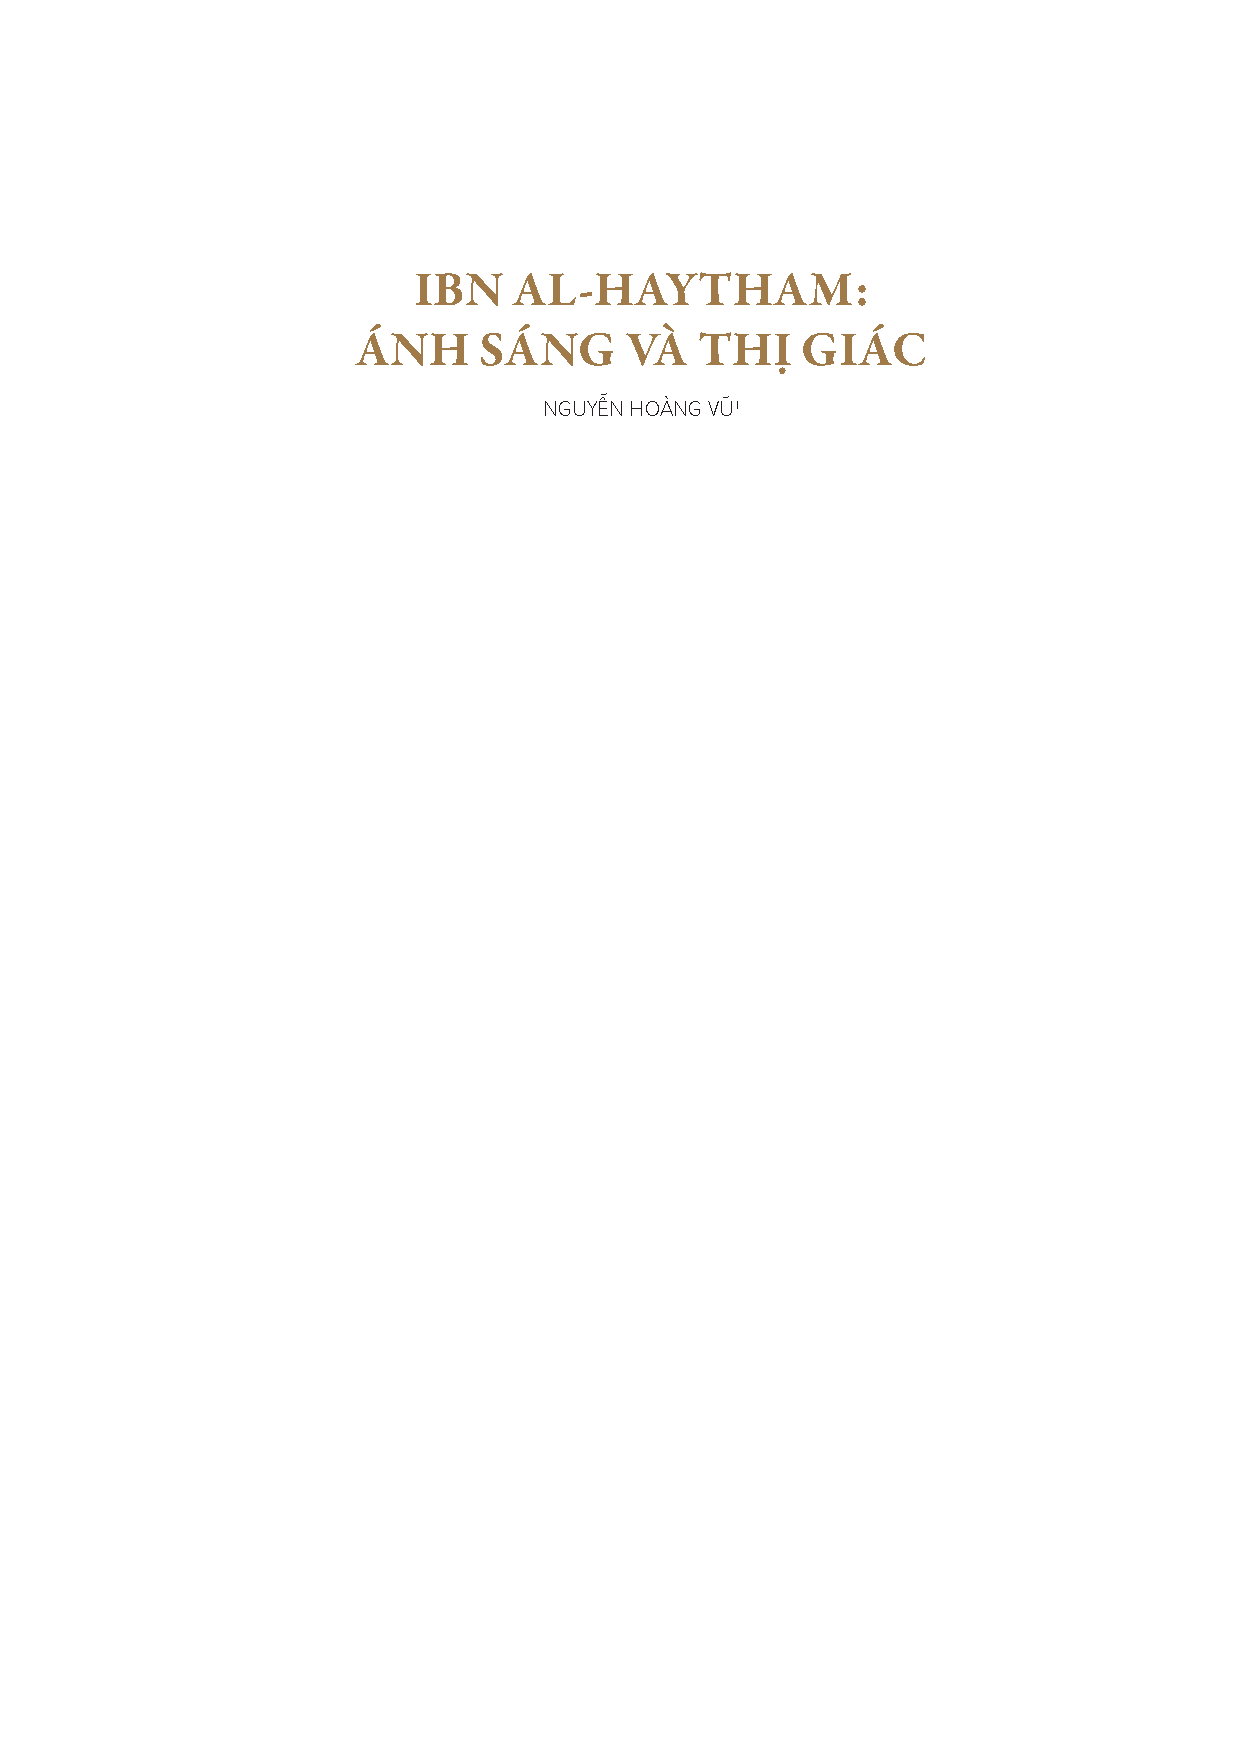
\includegraphics[scale=1]{../tieude.pdf}}}
\centering
\endgroup

\vspace*{185pt}

\begin{multicols}{2}
	Tại sao mắt người lại có thể nhìn thấy sự vật hiện tượng? Nhân loại đã mất đến hơn $1000$ nghìn năm cho đến khi Ibn al--Haytham, một học giả ở Cairo tìm ra câu trả lời cho vấn đề này. Trong bài viết này, chúng ta hãy cùng tìm hiểu về cuộc đời cùng những cống hiến cho khoa học của ông.
	\vskip 0.1cm
	$\pmb{1.}$ \textbf{\color{lichsutoanhoc}Quang học thời Hy Lạp cổ đại}
	\vskip 0.1cm
	Vào thời Hy Lạp cổ đại, cùng với sự phát triển của toán học thì việc xây dựng những lý thuyết về các hiện tượng tự nhiên cũng bắt đầu nảy sinh. Nhiều giả thuyết khác nhau được đưa ra trong giai đoạn này để giải thích một trong những vấn đề cơ bản nhất của quang học: tại sao các sự vật lại xuất hiện trong mắt của người nhìn.
	\vskip 0.1cm
	Leucippus và Democritus, các nhà triết học của thuyết nguyên tử, đề xuất rằng các eidolon, những bản sao mỏng cỡ nguyên tử của một vật thể, sẽ liên tục bay ra khỏi vật, đi qua không khí đến mắt người, nơi thị giác xảy ra. Trong khi đó, Aristotle cho rằng các loại vật chất phát ra từ mắt, kết hợp với ánh sáng từ ngọn lửa hoặc mặt trời, sẽ làm cho môi trường trở nên trong suốt và cho phép màu sắc từ vật đến mắt (màu sắc được Aristotle coi là một loại vật chất khác biệt với ánh sáng).
	\begin{figure}[H]
		\vspace*{5pt}
		\centering
		\captionsetup{labelformat= empty, justification=centering}
		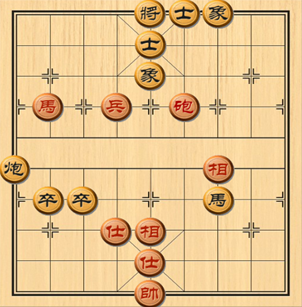
\includegraphics[width= 1\linewidth]{1}
		\caption{\small\textit{\color{lichsutoanhoc}Hình $1$. Một minh họa hình nón thị giác cho sách Quang học của Euclid phiên bản châu Âu.}}
		\vspace*{-10pt}
	\end{figure}
	Mặt khác, nhà toán học Euclid của chúng ta, từ các quan sát rằng mắt của động vật sáng lên trong bóng tối, lại cho rằng các tia thị giác được phát ra từ mắt, theo dạng một hình nón hình học với đỉnh là mắt và đáy hình nón nằm ở vật thể. Các tia này sẽ quét vật thể giống như radar ngày nay. Ông giải thích rằng các vật thể giao cắt với nhiều tia hơn sẽ trông lớn hơn và ngược lại. Những vật quá nhỏ sẽ nằm lọt giữa các tia và do đó sẽ không bị nhìn thấy.
	\vskip 0.1cm
	Một dạng giả thuyết thứ ba cho rằng có một loại ``khí thị giác" thoát ra từ não bộ vào mắt và đi ra thế giới bên ngoài. Giả thuyết này được ủng hộ bởi Galen, một thầy thuốc và nhà giải phẫu học Hy Lạp sống ở thế kỷ I sau Công nguyên.
	\vskip 0.1cm
	Các nhà toán học cho rằng thuyết eidolon không đúng do eidolon từ các ngôi nhà lớn hoặc ngọn núi không thể nào chui vừa vào con ngươi của mắt. Ngược lại, nhiều người cho rằng Euclid sai bởi nếu các tia phát ra từ mắt thì tại sao con người lại không nhìn thấy trong bóng tối. Nhà toán học Ptolemy thì cho rằng các tia thị giác của Euclid được phát ra liên tục trong toàn bộ hình nón chứ không rời rạc và các vật kích thích lên mắt người giống như việc sờ nắm kích thích xúc giác vậy. Cuộc tranh luận về cơ chế mắt người nhìn thấy vật kéo dài suốt vài trăm năm mà không có kết quả. 
	\vskip 0.1cm 
	$\pmb{2.}$ \textbf{\color{lichsutoanhoc}Quang học của al--Haytham}
	\vskip 0.1cm
	Phải hơn một nghìn năm sau Euclid, vấn đề cơ bản nêu trên về thị giác mới được Hasan Ibn al--Haytham, một học giả Arab giải quyết.
	\begin{figure}[H]
		\vspace*{-5pt}
		\centering
		\captionsetup{labelformat= empty, justification=centering}
		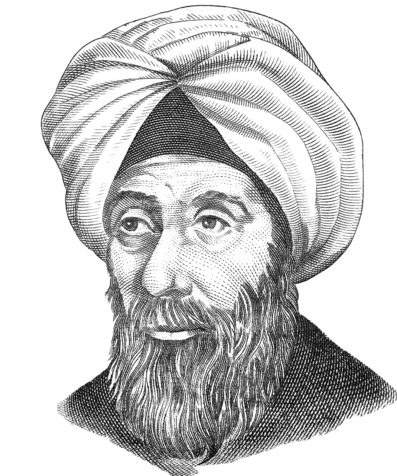
\includegraphics[width= 0.7\linewidth]{2}
		\caption{\small\textit{\color{lichsutoanhoc}Hasan Ibn al--Haytham ($965-1040$).}}
		\vspace*{-10pt}
	\end{figure}
	Al--Haytham sinh năm $965$ ở Basra, nay thuộc Iraq. Ông theo học ở đây cũng như ở Baghdad, trung tâm văn hóa và tri thức của thế giới Hồi giáo lúc đó. Do cảm thấy chán nản với những xung đột tôn giáo của xã hội lúc bấy giờ, ông không theo đuổi các lĩnh vực triết học tôn giáo và thần học như nhiều học giả Arab khác mà dành toàn bộ thời gian cho toán học và vật lý.
	\vskip 0.1cm
	Nhờ sự nổi tiếng về học thuật của mình, al--Haytham được al--Hakim, Caliph của khu vực Ai Cập lúc đó, mời sang giúp trị thủy sông Nile với tham vọng đưa vị thế của Ai Cập, dưới sự lãnh đạo của những người dòng Hồi giáo Shiite, vượt lên trên các thế lực Hồi giáo khác.
	\begin{figure}[H]
		\vspace*{-5pt}
		\centering
		\captionsetup{labelformat= empty, justification=centering}
		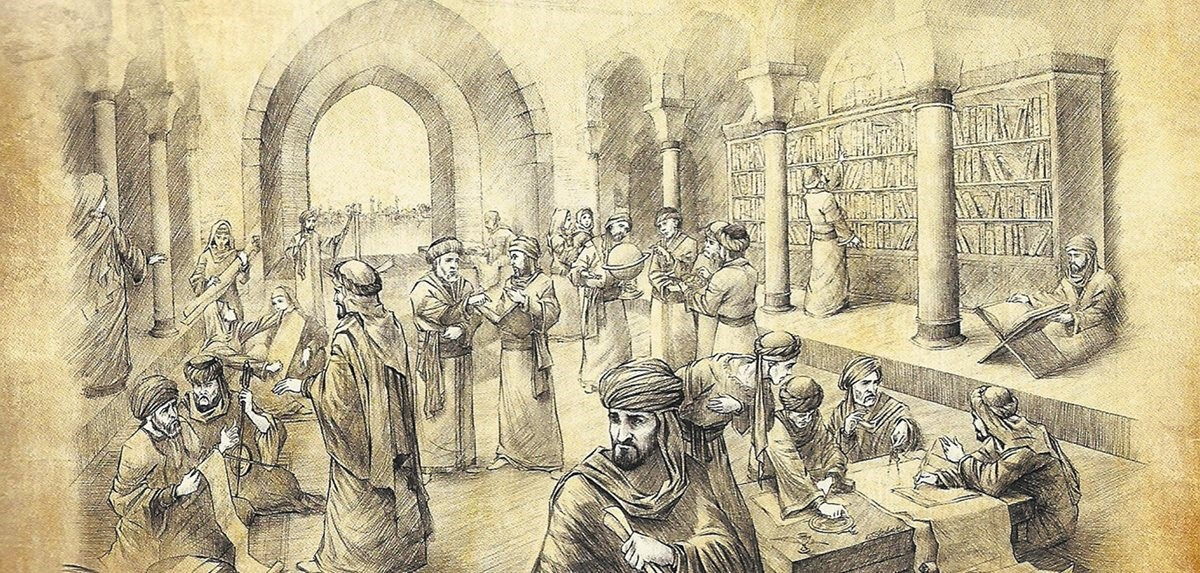
\includegraphics[width= 1\linewidth]{3}
		\caption{\small\textit{\color{lichsutoanhoc}Hình $2$. Thư viện ở Cairo do al--Hakim thành lập theo mô hình của thư viện ở Baghdad. Nhiều học giả được thu hút đến đây, trong đó có cả al--Haytham.}}
		\vspace*{-10pt}
	\end{figure}
	Phương án xây một con đập tại Aswan thượng nguồn sông Nile của al--Haytham được al--Hakim chấp thuận. Tuy nhiên, sau một thời gian, al--Haytham nhận thấy dự án này là bất khả thi với những tài nguyên mà ông có. Phải biết rằng, ngay cả với những phương pháp xây dựng và trang thiết bị hiện đại, con đập đầu tiên trên sông Nile cũng chỉ được hoàn thành vào năm $1902$, cao $36$ mét và dài $2000$ mét. Lo sợ bị trừng phạt bởi al--Hakim, một nhà lãnh đạo nổi tiếng về tính khí thất thường, al--Haytham đã nghĩ ra một biện pháp: giả điên. Ông bị giảm lỏng trong nhà ở Cairo trong suốt 10 năm cho đến khi vị Caliph bị ám sát. Sau khi được trả tự do, al--Haytham quay trở lại cuộc sống dạy học và viết sách. Trong giai đoạn bị trói buộc cũng như thời gian sau đó, gần như toàn bộ thời gian của al--Haytham được dùng để khám phá lĩnh vực quang học.
	\vskip 0.1cm
	Các nghiên cứu của al--Haytham được ghi lại chủ yếu trong cuốn sách \textit{Kitab al--Manazi} (Sách về Quang học) của ông. Trong đó, al--Haytham trình bày một giải thích đơn giản hơn về thị giác, thoát khỏi sự rắm rối của các lý thuyết từ thời Hy Lạp cổ đại. Theo ông, các tia sáng xuất phát từ các sự vật thay vì xuất phát từ mắt người như Euclid đã nói. Ánh sáng có thể được vật thể phát ra trực tiếp (nguồn sáng sơ cấp như mặt trời, ngọn lửa) hoặc cũng có thể là ánh sáng được vật phản xạ lại (nguồn sáng thứ cấp). Tia sáng truyền đi theo đường thẳng đến mắt nếu không có vật khác chắn ở giữa. Những lý thuyết trên đều được al--Haytham xây dựng trên cơ sở các lập luận và thí nghiệm thực tế. 
	\begin{figure}[H]
		\vspace*{-5pt}
		\centering
		\captionsetup{labelformat= empty, justification=centering}
		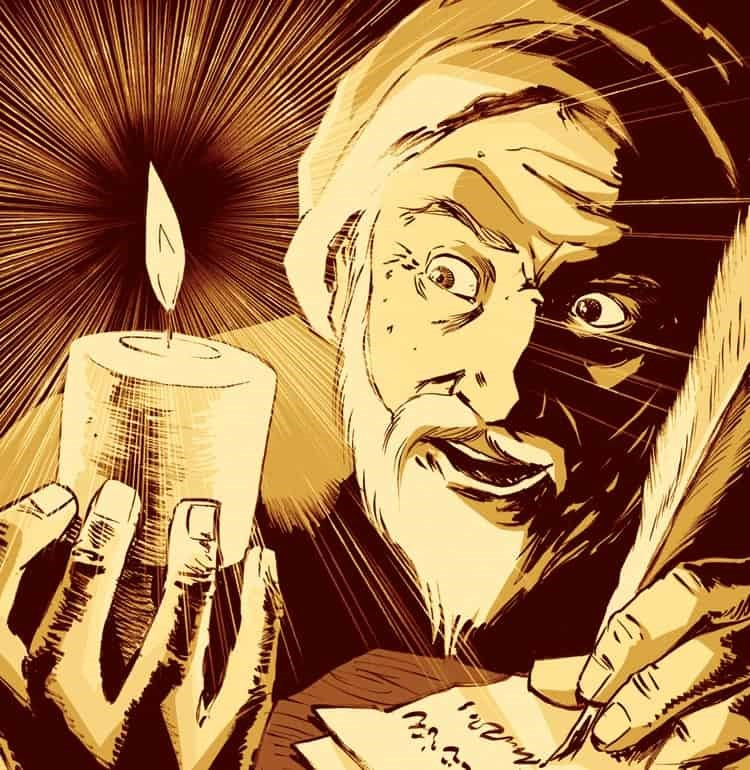
\includegraphics[width= 0.75\linewidth]{4}
		\caption{\small\textit{\color{lichsutoanhoc}Hình $3$. Minh họa al--Haytham nghiên cứu về các nguồn sáng.}}
		\vspace*{-10pt}
	\end{figure}
	Một sự thật đơn giản là khi một người nhìn thẳng vào mặt trời thì mắt sẽ bị đau. Vậy rõ ràng là ánh sáng từ mặt trời có tác động đến mắt chứ không phải tia sáng từ mắt đến mặt trời bởi nếu các tia sáng phát ra từ mắt thì chúng không thể lại gây tổn thương cho mắt được. Đồng thời, nếu ta nhìn thấy vật thể bởi vi mắt phát ra các tia đến vật đó thì khi ta nhìn thấy các vì sao, các tia vật chất này cũng lấp đầy không gian giữa ta và các ngôi sao ở rất xa?
	\vskip 0.1cm
	Mặt khác, nếu tia sáng đi từ mắt đến vật như Euclid nói thì vật có gửi lại tín hiệu về mắt không? Nếu không, thì làm sao mắt có thể biết các tia của mình chạm vào vật nào? Nếu có, thì có nghĩa là ta cần có tia sáng đi từ vật đến mắt để có thể nhìn thấy. Như vậy thì giải thích rằng vật thể là nguồn sáng sẽ thích hợp hơn bởi ta đã biết mắt không thể nhìn thấy trong bóng tối khi không có nguồn sáng nào.
	\vskip 0.1cm
	Al--Haytham cũng đã tiến hành các thí nghiệm công phu để khẳng định rằng ánh sáng truyền đi theo đường thẳng. Với ánh sáng từ mặt trời (thuộc dạng nguồn sáng sơ cấp), ông tiến hành đục một lỗ ở trên bức tường ngăn cách hai ngôi nhà, một ở phía đông và một ở phía tây. Vào lúc bình minh, ánh sáng chiếu từ một lỗ khác trên tường phía đông của ngôi nhà phía đông sẽ xuyên qua lỗ ở tường ngăn cách và điểm được chiếu sáng ở ngôi nhà phía tây sẽ thẳng hàng với hai lỗ này. Khi đặt một vật chắn thì ánh sáng sẽ không chiếu vào tường nữa mà sẽ vệt sáng sẽ xuất hiện trên vật. Ông cũng lặp lại các thí nghiệm này với ánh sáng từ mặt trăng và sao Kim. Đồng thời, khi các nguồn sáng trên chuyển động thì vệt sáng do ánh sáng xuyên qua lỗ trên tường tạo thành cũng sẽ chuyển động tương ứng sao cho các lỗ và vệt sáng luôn thẳng hàng.Thí nghiệm tương tự với ánh sáng từ ngọn nến cũng cho thấy sự thẳng hàng này. Tính truyền thẳng của ánh sáng phản xạ còn được khẳng định bằng việc quan sát một bức tường trắng từ hai lỗ trên bức tường đối diện. Hai lỗ này được khoan sao cho đường kéo dài của chúng cùng hội tụ tại một điểm ở trên bức tường trắng. Khi quan sát từ bất kỳ lỗ nào cũng đều thấy điểm hội tụ này.
	\begin{figure}[H]
		\vspace*{-10pt}
		\centering
		\captionsetup{labelformat= empty, justification=centering}
		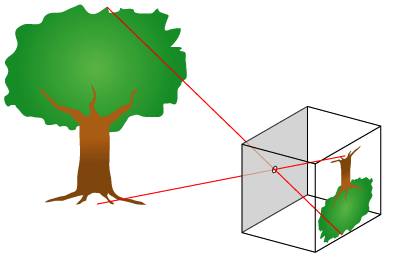
\includegraphics[width= 1\linewidth]{5}
		\caption{\small\textit{\color{lichsutoanhoc}Hình $4$. Minh họa cơ chế tạo ảnh của camera obscura. Buồng tối có thể là một căn phòng hay một hộp giấy.}}
		\vspace*{-5pt}
	\end{figure}
	Al--Haytham rất chú trọng đến các dụng cụ làm thí nghiệm và mô tả chi tiết trong cuốn sách cách chế tạo cũng như sử dụng chúng. Một dụng cụ thí nghiệm tương đối nổi tiếng mà al--Haytham sử dụng là thiết bị mà sau này các học giả phương Tây gọi là camera obscura. Nó gồm một buồng tối có đục một lỗ rất nhỏ. Ở trên một tấm màn đối diện, sẽ xuất hiện ảnh của vật bên ngoài theo chiều ngược lại. Hiện tượng này thể hiện rõ rệt sự truyền thẳng của ánh sáng. Trong trường hợp lỗ quá to thì ảnh sẽ bị mờ hoặc biến mất do mỗi điểm trên màn nhận được tia sáng từ rất nhiều điểm khác nhau ở bên ngoài. Tuy al--Haytham không phải là người đầu tiên phát minh ra camera obscura, ông là người đầu tiên đưa ra giải thích bằng mô hình hình học về cơ chế hoạt động của nó. Các bạn học sinh cũng có thể tự làm một camera obscura ở nhà bằng cách đục lỗ trên một hộp giấy và thay phần bìa ở phía đối diện lỗ bằng giấy can làm màn quan sát.
	\begin{figure}[H]
		\vspace*{-5pt}
		\centering
		\captionsetup{labelformat= empty, justification=centering}
		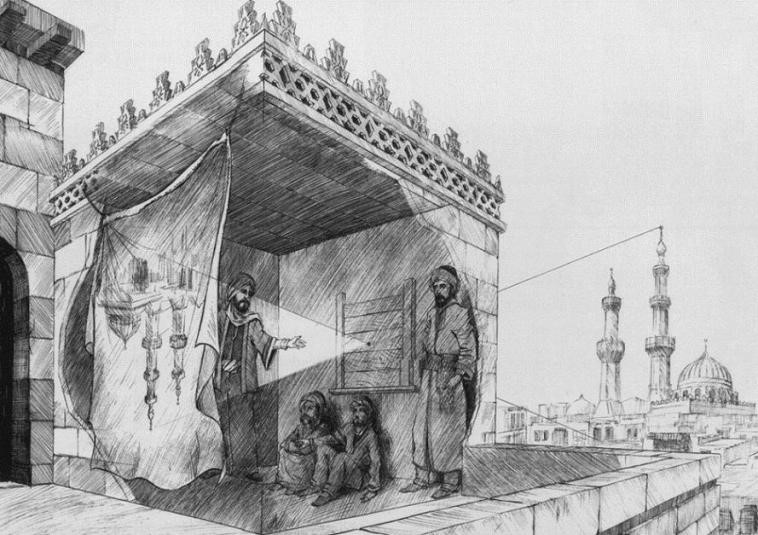
\includegraphics[width= 1\linewidth]{6}
		\caption{\small\textit{\color{lichsutoanhoc}Hình $5$. al--Haytham và camera obscura.}}
		\vspace*{-10pt}
	\end{figure}
	Không chỉ thiết lập lại đúng chiều và phương thức truyền đi của ánh sáng, al--Haytham cũng đưa ra một mô hình mới về thị giác. Ông đã xác định được rằng thủy tinh thể đóng vai trò của một thấu kính mà ảnh qua nó sẽ được hệ thần kinh tiếp nhận. Sau đó, thông tin từ cả hai mắt sẽ được bộ não xử lý để cho ra hình ảnh. Các chi tiết trong mô hình của ông còn có nhiều điểm thiếu sót mà sau này khoa học mới dần khám phá hết nhưng về cơ bản, al-Haytham đã có một mô hình đầu tiên giải thích một cách khoa học cách thức mà con người có thể nhìn thấy thế giới này. Ông cũng nghiên cứu các thông số của mắt như điểm cực cận, điểm cực viễn và độ phân giải của thị giác.
	\begin{figure}[H]
		\vspace*{-5pt}
		\centering
		\captionsetup{labelformat= empty, justification=centering}
		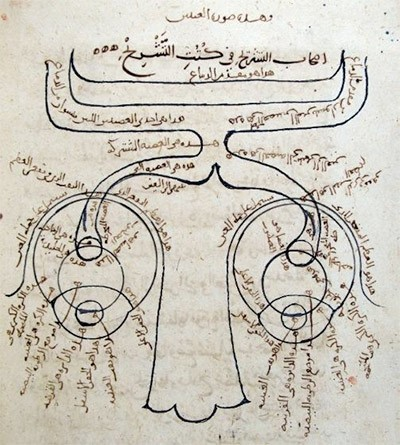
\includegraphics[width= 1\linewidth]{7}
		\caption{\small\textit{\color{lichsutoanhoc}Hình $6$. Mô tả của al--Haytham về vai trò của mắt trong thị giác.}}
		\vspace*{-10pt}
	\end{figure}
	Al--Haytham còn nghiên cứu nhiều vấn đề khác của quang học như các hiện tượng phản xạ, khúc xạ ánh sáng, cầu vồng và các hiện tượng quang học khác trong tự nhiên. Một hiện tượng mà ông rất quan tâm là việc mặt trăng khi ở gần đường chân trời sẽ trông lớn hơn so với khi nó ở trên cao. Hiện tượng này đã được ghi chép lại từ thời cổ đại ở nhiều nền văn minh khác nhau. Bản thân Ptolemy cũng như nhiều học giả Hy Lạp cho rằng nguyên nhân của việc này là do khúc xạ ánh sáng trong khí quyển. Tuy nhiên thực tế không phải như vậy. Tính toán hiện đại cho thấy khúc xạ chỉ thay đổi kích thước mặt trăng có $1,5\%$ mà thôi. Nếu ta chụp hai tấm ảnh của mặt trăng ở hai vị trí trên và đo thì có thể thấy kích thước mặt trăng thật sự không thay đổi. Al--Haytham là người đầu tiên kiểm chứng từ đo đạc thực nghiệm rằng hiện tượng này là do ảo giác chứ không phải một hiện tượng vật lý. Khi mặt trăng ở trên cao, mắt ta không có vật thể nào để làm tham chiếu nhưng khi nó ở gần chân trời, những vật thể xung quanh như ngọn núi, cây cối, ngôi nhà có thể gây ra cảm nhận thị giác khác biệt về mặt kích thước.
	\begin{figure}[H]
		\vspace*{-5pt}
		\centering
		\captionsetup{labelformat= empty, justification=centering}
		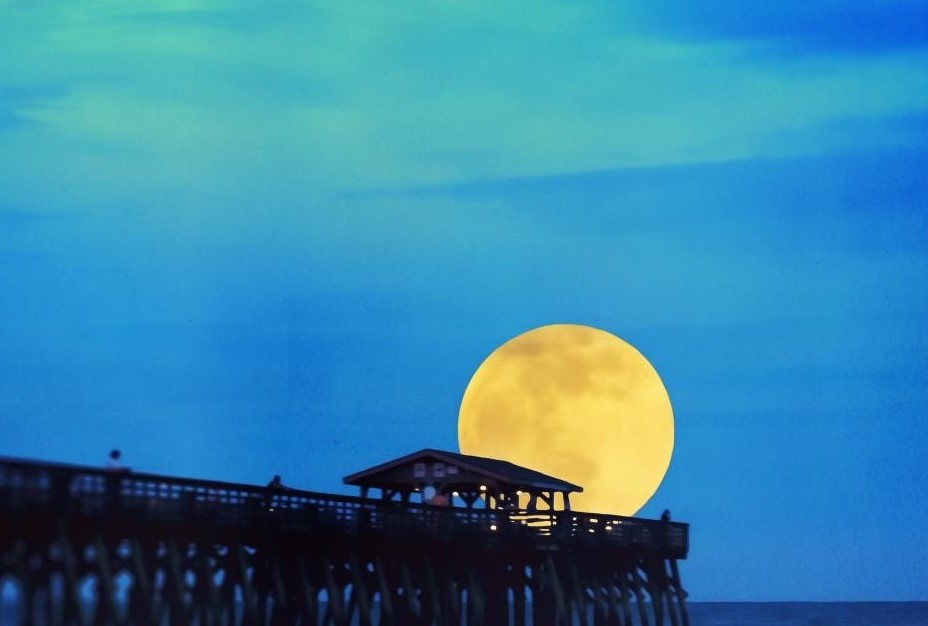
\includegraphics[width= 1\linewidth]{8}
		\caption{\small\textit{\color{lichsutoanhoc}Hình $7$. Khi ở gần đường chân trời, mặt trăng trông có vẻ to hơn nhiều so với khi nó ở trên cao.}}
		\vspace*{-10pt}
	\end{figure}
	Vào thế kỷ $12$ và thế kỷ $13$, khi nhiều cuốn sách khoa học được dịch từ tiếng Arab sang tiếng Latin, al--Haytham được biết đến với tên Latin là al--Hazen. Tác phẩm của al--Hazen trở thành cơ sở kiến thức quang học cho các nghiên cứu của những nhà khoa học phương Tây thế kỷ $13$ như Roger Bacon và Witelo. Hơn thế nữa, việc sử dụng thí nghiệm để kiểm chứng mô hình lý thuyết mà al--Hazen chú trọng có ảnh hưởng lớn đến sự phát triển của vật lý, trong cả cơ học của Galileo lẫn quang học của Kepler và Newton sau này. Có thể nói, al--Hazen là một nhà khoa học đầu tiên trong lịch sử, theo đúng quy trình của phương pháp khoa học: ông sử dụng lý thuyết để giải thích kết quả thực nghiệm và sử dụng thí nghiệm để kiểm chứng mô hình lý thuyết. Ông đã đưa khoa học thoát khỏi tính siêu hình và trừu tượng của các lập luận Hy Lạp để đưa nó đến gần với thực tế tự nhiên hơn. Một chi tiết đáng chú ý là đến tận đầu thế kỷ $20$, từ những bản thảo tiếng Arab phát hiện được, người ta mới biết al--Hazen và al--Haytham là cùng một người.
	\begin{figure}[H]
		\vspace*{5pt}
		\centering
		\captionsetup{labelformat= empty, justification=centering}
		
\includegraphics[width= 1\linewidth]{9}
		\caption{\small\textit{\color{lichsutoanhoc}Hình $8$. al--Hazen (trái) và Galileo (phải) trên bìa một cuốn sách thế kỷ $17$. Trước khi có các phát hiện của Kepler và Newton, các cuốn sách al--Hazen và Galileo được coi là những tài liệu kinh điển của lĩnh vực vật lý ở châu Âu.}}
		\vspace*{-10pt}
	\end{figure}
	$\pmb{3.}$ \textbf{\color{lichsutoanhoc}Bài toán al--Hazen}
	\vskip 0.1cm
	Toán học của Al--Haytham về cơ bản thừa kế từ các tác giả Hy Lạp cổ đại như Euclid, Ptolemy và Apollonius. Ông sử dụng những kiến thức toán học này để giải quyết các vấn đề liên quan đến quang học. Đặc biệt, các đường conic được dùng để giải các bài toán quang học phức tạp.
	\vskip 0.1cm
	Bài toán nổi tiếng nhất của al--Haytham, được đặt tên là bài toán al-Hazen, có nội dung như sau:
	\vskip 0.1cm
	``Một vật thể và một người quan sát có các vị trí cho trước trong mặt phẳng. Hãy xác định các điểm trên một vành gương tròn sao cho tia sáng từ vật thể phản xạ tại điểm này sẽ đến người quan sát".
	\vskip 0.1cm
	Bài toán trên được Ptolemy phát biểu từ trước đó nhưng al--Haytham là người tìm ra cách giải. Ông đã sử dụng các đường conic để giải bài toán này cũng như trường hợp mở rộng cho mặt cầu và mặt nón trong không gian ba chiều. Những lời giải bằng hình học này rất phức tạp và dài. Đến thế kỷ $17$, với sự ra đời của hình học giải tích, nhiều nhà toán học đã đi tìm cách giải khác sử dụng các phương pháp tọa độ của Descartes. Trong khi nhà toán học Sluse dùng đường parabola thì Huygens cho ra lời giải sử dụng đường hyperbola. Một cách giải bằng số phức được trình bày trong phần phụ lục.
	\begin{figure}[H]
		\vspace*{-10pt}
		\centering
		\captionsetup{labelformat= empty, justification=centering}
		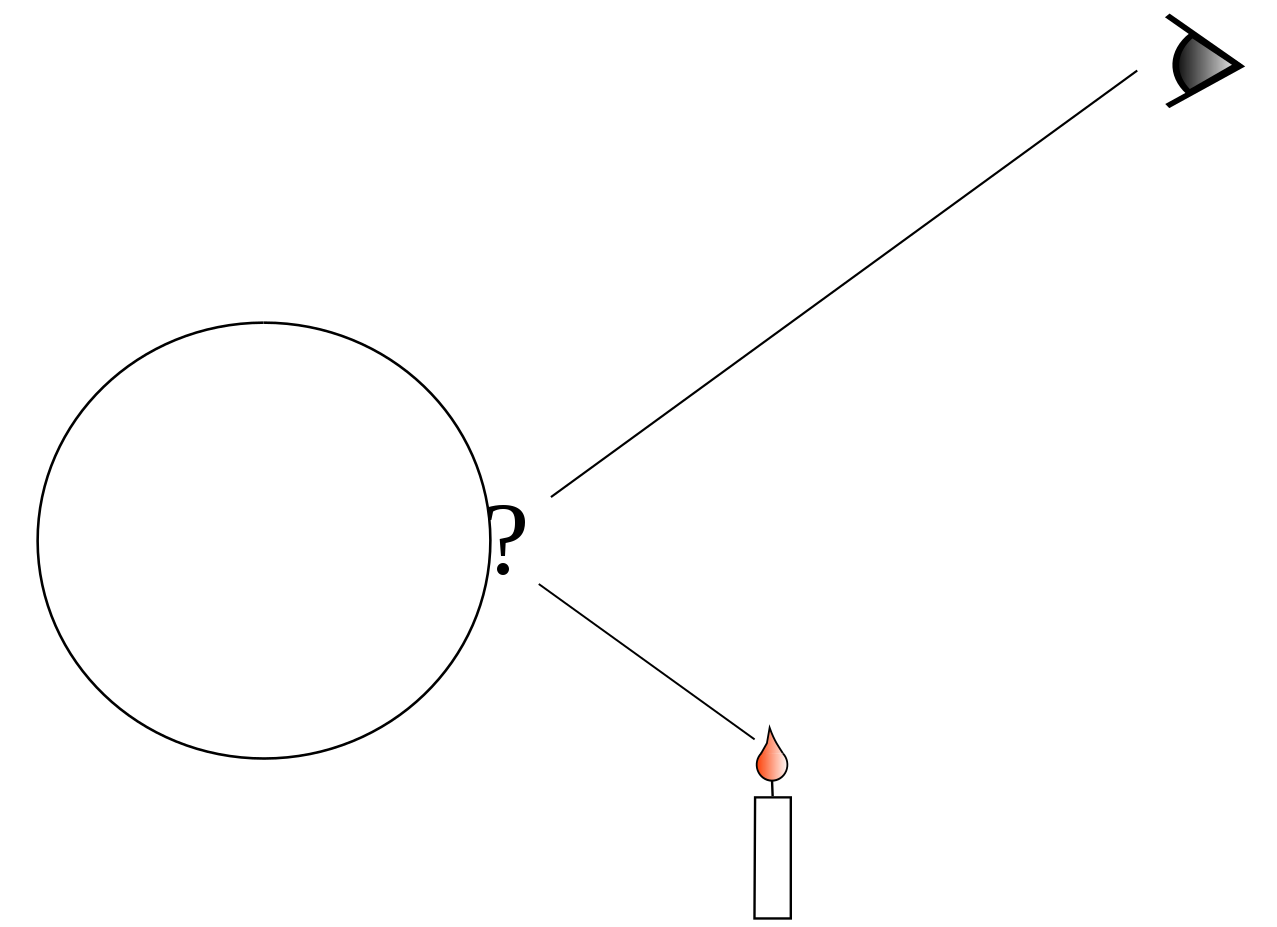
\includegraphics[width= 1\linewidth]{10}
		\caption{\small\textit{\color{lichsutoanhoc}Hình $9$. Bài toán al--Hazen.}}
		\vspace*{-10pt}
	\end{figure}
	Bài toán al--Hazen cùng trường hợp mở rộng cho hình cầu của nó vẫn đang là đề tài của nhiều nghiên cứu trong toán học và các ngành khoa học khác như đồ họa máy tính, phản xạ trong khí quyển, ...
	\vskip 0.1cm
	$\pmb{4.}$ \textbf{\color{lichsutoanhoc}Lời kết}
	\vskip 0.1cm
	Ngay từ thế kỷ thứ $10$, al--Haytham và các học giả cùng thời khác như Ibn Sina và al--Biruni đã thảo luận những vấn đề rất hiện đại như ánh sáng là liên tục hay rời rạc; hoặc vận tốc ánh sáng có hữu hạn hay không. Họ gần với chúng ta hơn nhiều so với những gì chúng ta vẫn tưởng. Tuy nhiên, do sự thắng thế của các tư tưởng bảo thủ cũng như những cuộc xâm lược bên ngoài từ người Mông Cổ, sự phát triển của khoa học trong thế giới Hồi giáo đã bị dừng lại. Trong khi đó, những tư tưởng mà al--Haytham cùng nhiều học giả Trung đông khác xây dựng trên cơ sở toán học Hy Lạp lại được châu Âu tiếp thu trong giai đoạn trước và trong thời Phục Hưng, làm tiền đề cho cuộc cách mạng khoa học thế kỷ $17$ với các tên tuổi như Galileo, Kepler và Newton. Lịch sử của quang học nói riêng và khoa học nói chung còn nhiều đề tài rất thú vị mà Pi sẽ chuyển tải đến độc giả trong các số sau.
	\begin{figure}[H]
		\vspace*{-5pt}
		\centering
		\captionsetup{labelformat= empty, justification=centering}
		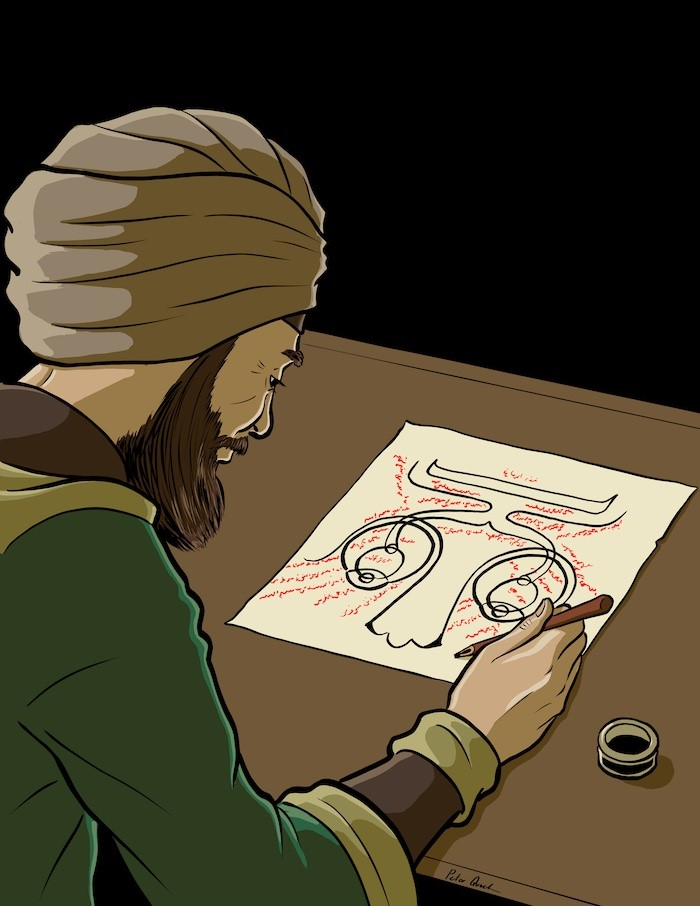
\includegraphics[width= 0.85\linewidth]{11}
		\vspace*{-5pt}
	\end{figure}
	\textbf{\color{lichsutoanhoc}Phụ lục: Bài toán al--Hazen giải bằng số phức}
	\begin{figure}[H]
		\vspace*{-5pt}
		\centering
		\captionsetup{labelformat= empty, justification=centering}
		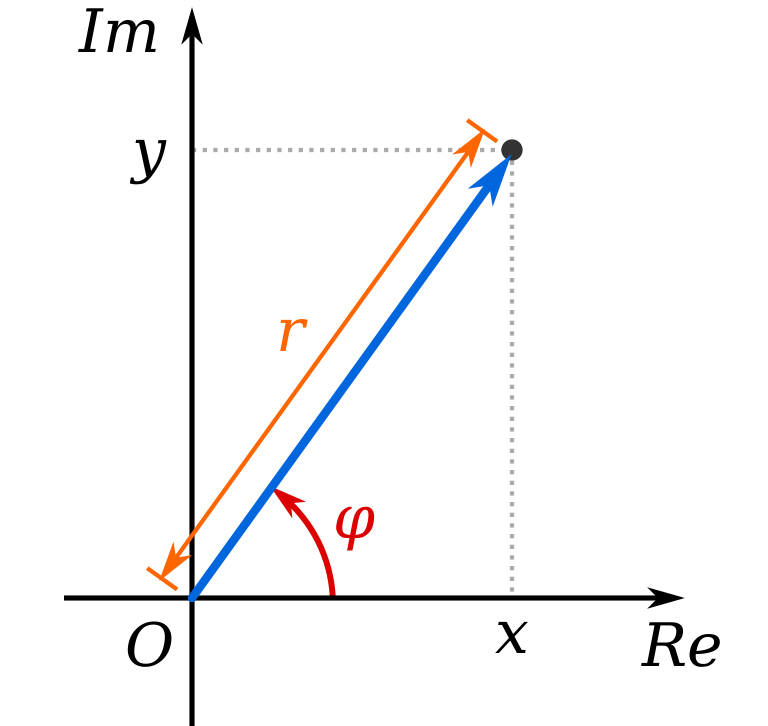
\includegraphics[width= 0.75\linewidth]{12}
		\caption{\small\textit{\color{lichsutoanhoc}Số phức biểu diễn theo dạng cực.}}
		\vspace*{-10pt}
	\end{figure}
	Trước khi giải bài toán al--Hazen, ta hãy tìm hiểu một số khái niệm liên đến số phức. Argument (viết tắt là arg) của một số phức $z$ là góc $\phi$ mà vector từ gốc tọa độ của mặt phẳng phức đến điểm biểu diễn $z$ tạo với trục thực. Số thực $x+i\cdot y$ sẽ có argument là $\tan^{-1}\frac{y}{x}$. Khi viết số thực dưới dạng cực, ta có: $x+i\cdot y=r(\cos\phi+i\cdot \sin\phi)=re^{i\phi}$.
	\vskip 0.1cm 
	Có thể dễ dàng chứng minh rằng khi nhân hai số phức viết theo dạng cực, $r_1 e^{i\phi_1}$ và $r_2 e^{i\phi_2}$ thì tích sẽ có độ lớn $r_1\cdot r_2$ và argument bằng $\phi_1 + \phi_2$. Cách biểu diễn dạng cực rất tiện lợi khi chứng minh hình học do bán kính và góc là các khái niệm cơ bản sẵn có của lĩnh vực này. Thay vì biểu diễn một điểm theo dạng $(x,y)$ trong tọa độ Descartes, ta biểu diễn nó bằng một số phức $z=x+i\cdot y$ có bán kính $r=\sqrt{x^2 + y^2}$ và $\phi = \tan^{-1}\frac{y}{x}$. Số phức $z$ và số phức liên hợp $\overline{z}$ của nó sẽ biểu diễn hai điểm đối xứng qua trục $x$. Góc cũng có thể được tính qua phép chia số phức: $\arg\frac{a}{b}$ sẽ là góc tạo bởi hai đường thẳng từ gốc tọa độ đến các điểm ứng với hai số phức $a$, $b$ trong mặt phẳng.
	\begin{figure}[H]
		\vspace*{-10pt}
		\centering
		\captionsetup{labelformat= empty, justification=centering}
		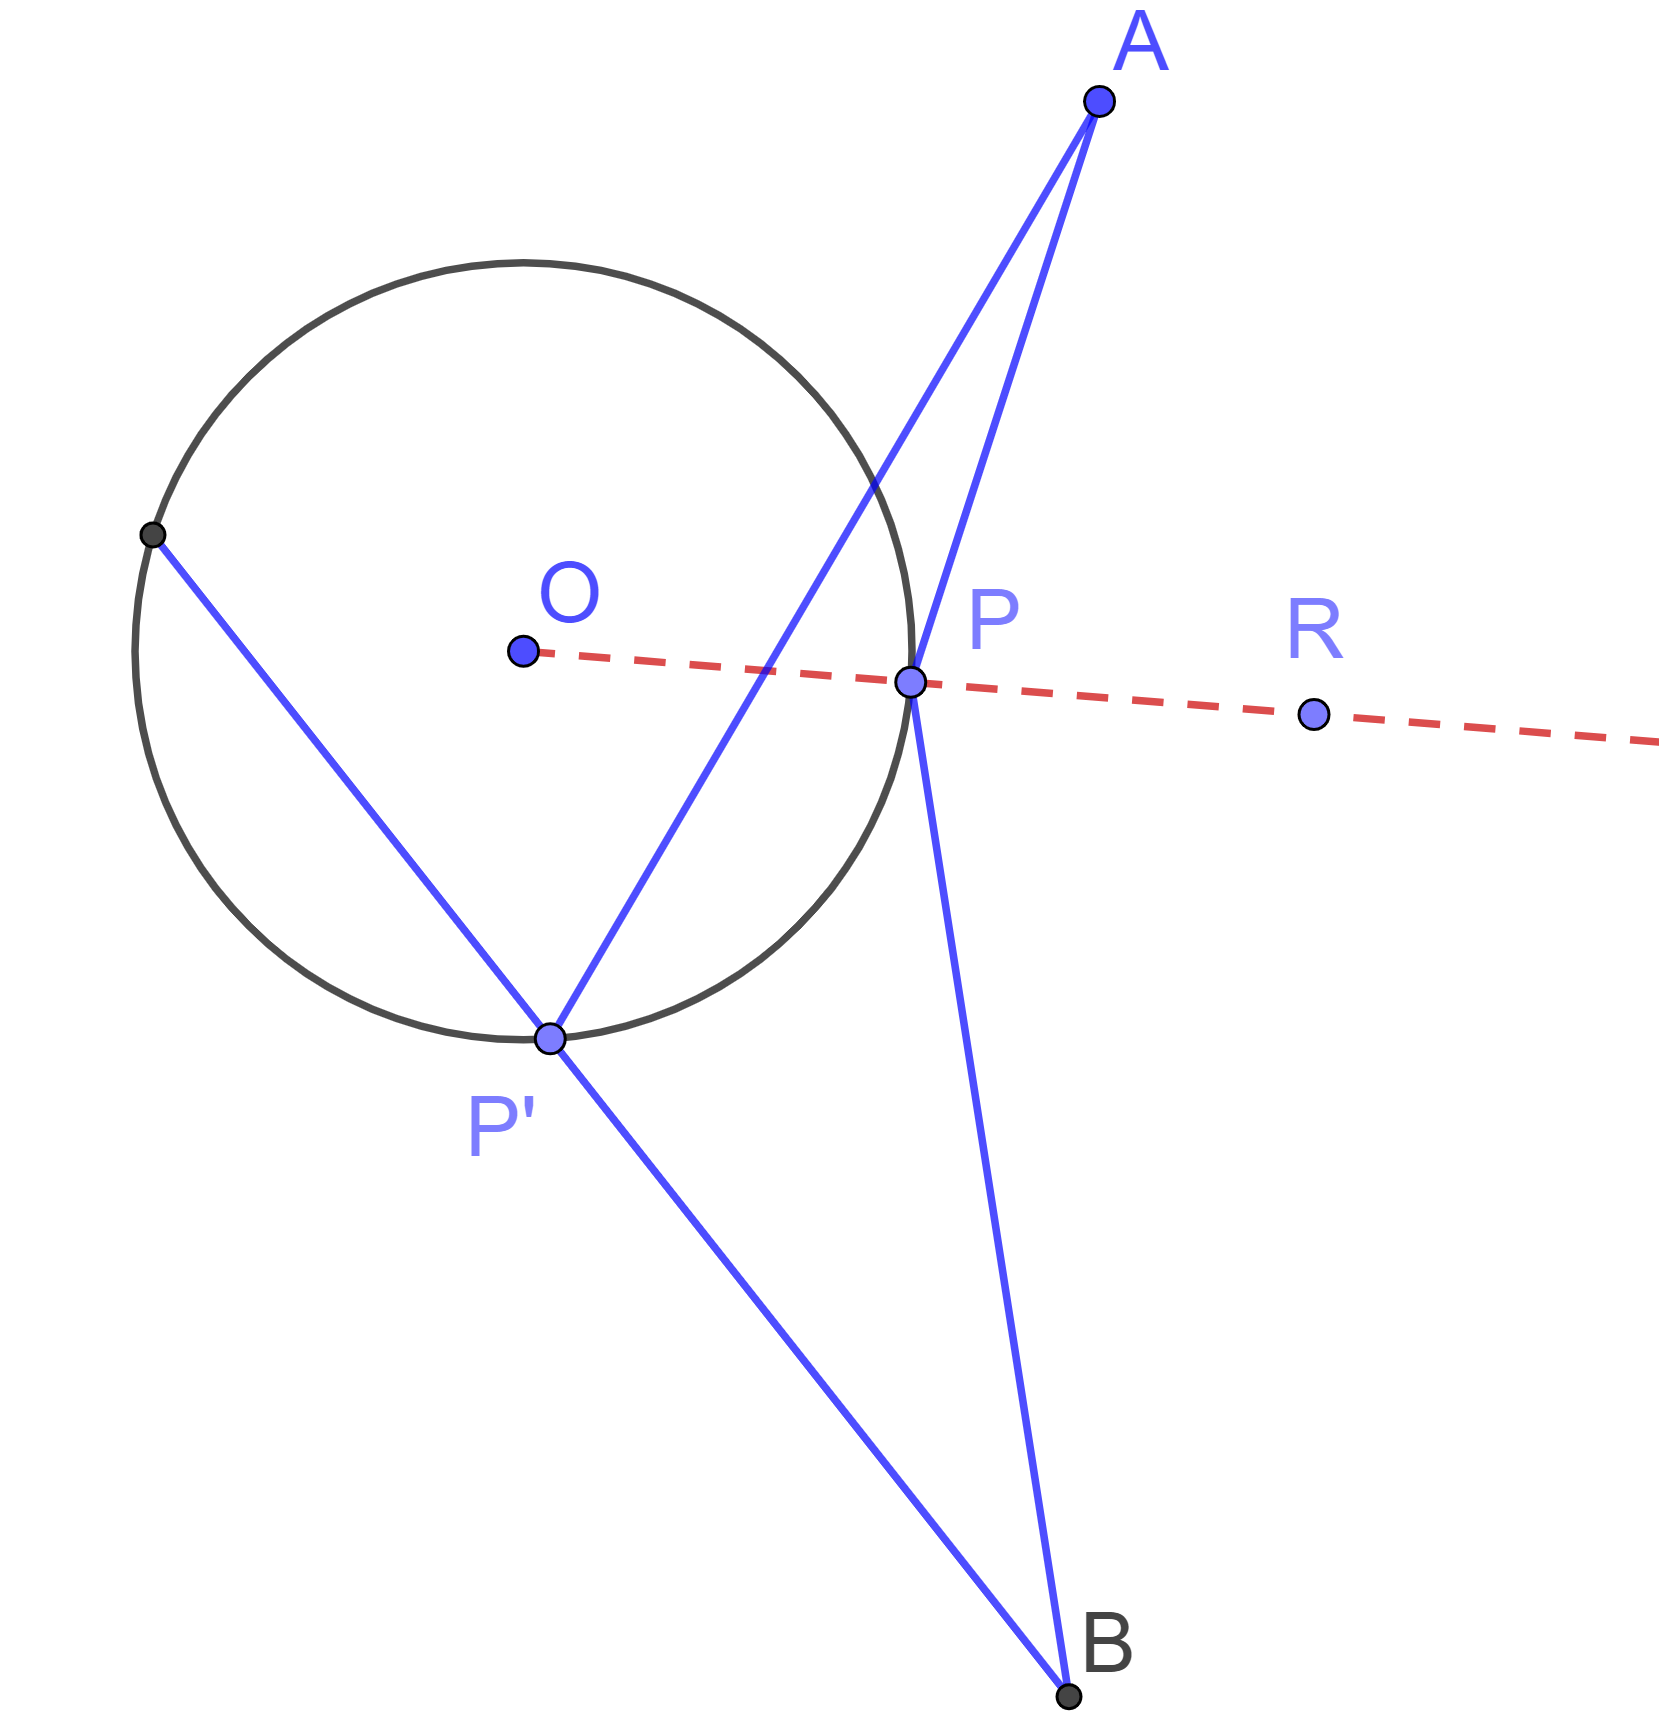
\includegraphics[width= 0.85\linewidth]{13}
		\caption{\small\textit{\color{lichsutoanhoc}Bài toán al--Hazen.}}
		\vspace*{-10pt}
	\end{figure}
	Trở lại bài toán toán al--Hazen, gọi $A$ là vị trí vật, $B$ là vị trí người quan sát. Vành tròn phản xạ có tâm ở $O$. $PR$ là pháp tuyến tại $P$. Tia sáng từ $A$ đến $P$ sẽ phản xạ sang $B$. Ta biểu diễn tọa độ của $A$, $B$ và $P$ bằng các số phức $a$, $b$ và $z$.
	\vskip 0.1cm
	Góc tới $APR$ và góc phản xạ $RPB$ có độ lớn bằng nhau và ngược chiều quay từ pháp tuyến nên:
	\begin{align*}
		\arg\left(\frac{a-z}{z}\right) = - \arg\left(\frac{b-z}{z}\right).
	\end{align*}
	Do đó:
	\begin{align*}
		\arg\left(\frac{(a-z)(b-z)}{z^2}\right) = 0 \tag{$1$}
	\end{align*}
	($1$) có nghĩa rằng biểu thức trong ngoặc ở trên là một số thực (argument bằng $0$ nên không có phần ảo). Do đó:
	\begin{align*}
		\frac{(a-z)(b-z)}{z^2} = \frac{(\overline{a}- \overline{z})(\overline{b}- \overline{z})}{\overline{z}^2} \tag{$2$}
	\end{align*}
	với $\overline{z}$ là liên hợp phức của $z$.
	\vskip 0.1cm
	Phương trình trên thỏa mãn khi hai góc $APR$ và $RPB$ bằng nhau hoặc khác nhau $\pi$. Như trong hình, tia $AP'$ có tia sáng phản xạ nằm trên đường thẳng $P'B$. Ta coi cả $P$ và $P'$ đều là điểm phản xạ cần tìm.
	\vskip 0.1cm
	Lấy các trục tọa độ của mặt phẳng là đường phân giác của góc $AOB$ và đường thẳng vuông góc với đường phân giác này, gốc tọa độ ở $O$, thì tích $ab$ sẽ là một số thực. Nhân chéo hai vế của ($2$) rồi chia cho $ab$ ta được:
	\begin{align*}
		z^2 - \overline{z}^2 = \left[(a^*+ b^*)z - \overline{(a^*+b^*)}\overline{z}\right]z\overline{z}
	\end{align*}
	với $a^*=\frac{1}{\overline{a}}$ và  $b^*=\frac{1}{\overline{b}}$. Đặt $c = \frac{1}{2}(a^*+ b^*)$ ta được:
	\begin{align*}
		z^2 - \overline{z}^2 = 2 (cz - \overline{c}\overline{z})z\overline{z}.
	\end{align*}
	Viết các số phức theo dạng $c = |c|e^{i\delta}$ và $z=re^{i\theta}$ ta được một đường cong phức dạng cực như sau:
	\begin{align*}
		r = \frac{\sin2\theta}{2|c|\sin(\theta + \delta)}. \tag{$3$}
	\end{align*}
	Đây là đường cong mà nhà toán học Isaac Barrow tìm ra năm $1669$.
	\begin{figure}[H]
		\vspace*{-5pt}
		\centering
		\captionsetup{labelformat= empty, justification=centering}
		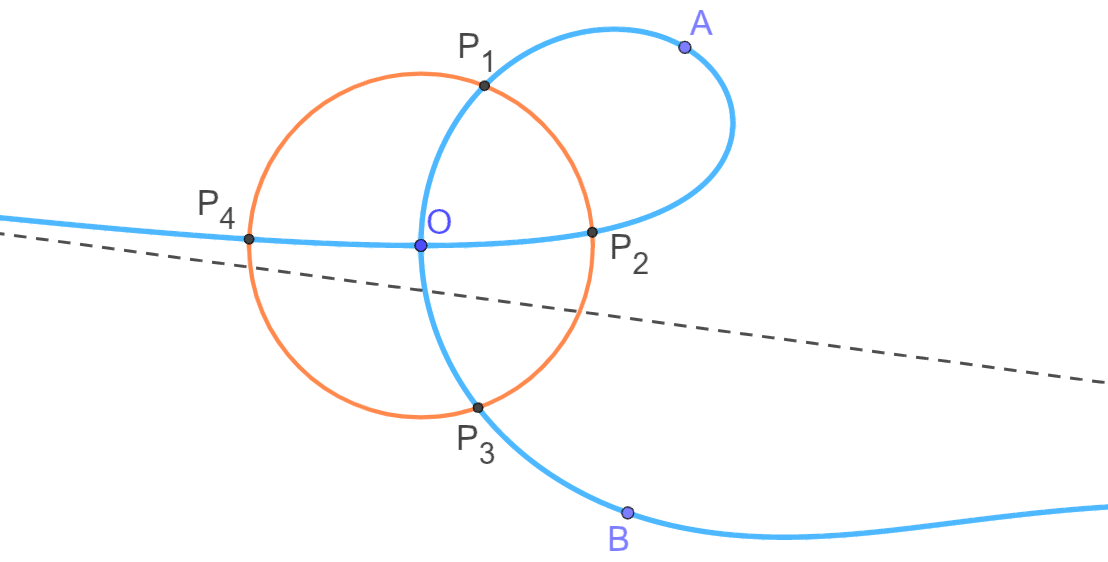
\includegraphics[width= 1\linewidth]{14}
		\caption{\small\textit{\color{lichsutoanhoc}Đường cong Barrow.}}
		\vspace*{-10pt}
	\end{figure}
	Thay $c=c_1+i\cdot c_2$, ta thu được biểu diễn của đường cong ($3$) trong mặt phẳng tọa độ Descartes:
	\begin{align*}
		xy = \left(c_2x + c_1y\right)\left(x^2 + y^2\right).
	\end{align*}
	Đường cong trên cho ta quỹ tích các điểm trong mặt phẳng sao cho các góc $APR$ và $BPR$ bằng nhau hoặc khác nhau $\pi$. Do $a$ và $b$ đều là nghiệm của ($2$) nên đường cong ($3$) đi qua $A$ và $B$. Vẽ đường tròn tâm $O$, bán kính bằng với bán kính của gương thì các giao điểm của đường tròn với đường cong ($3$) là các điểm phản xạ cần tìm. Số điểm phản xạ này sẽ thay đổi từ $2$ đến $4$ tùy theo bán kính đường tròn.
	\vskip 0.1cm
	Không làm mất tính tổng quát, giả sử gương là đường tròn đơn vị có $|z| = 1$. Khi đó,
	\begin{align*}
		xy = c_2x + c_1y
	\end{align*}
	và ta có:
	\begin{align*}
		\left(x-c_1\right)(y-c_2)= c_1c_2
	\end{align*}
	hay
	\begin{align*}
		y = \frac{c_1c_2}{x - c_1} + c_2.
	\end{align*}
	Có nghĩa là, các điểm $P$ ta cần tìm là giao điểm của đường tròn với hai nhánh hyperbola có các tiệm cận $x=c_1$ và $y=c_2$.
	\begin{figure}[H]
		\vspace*{-5pt}
		\centering
		\captionsetup{labelformat= empty, justification=centering}
		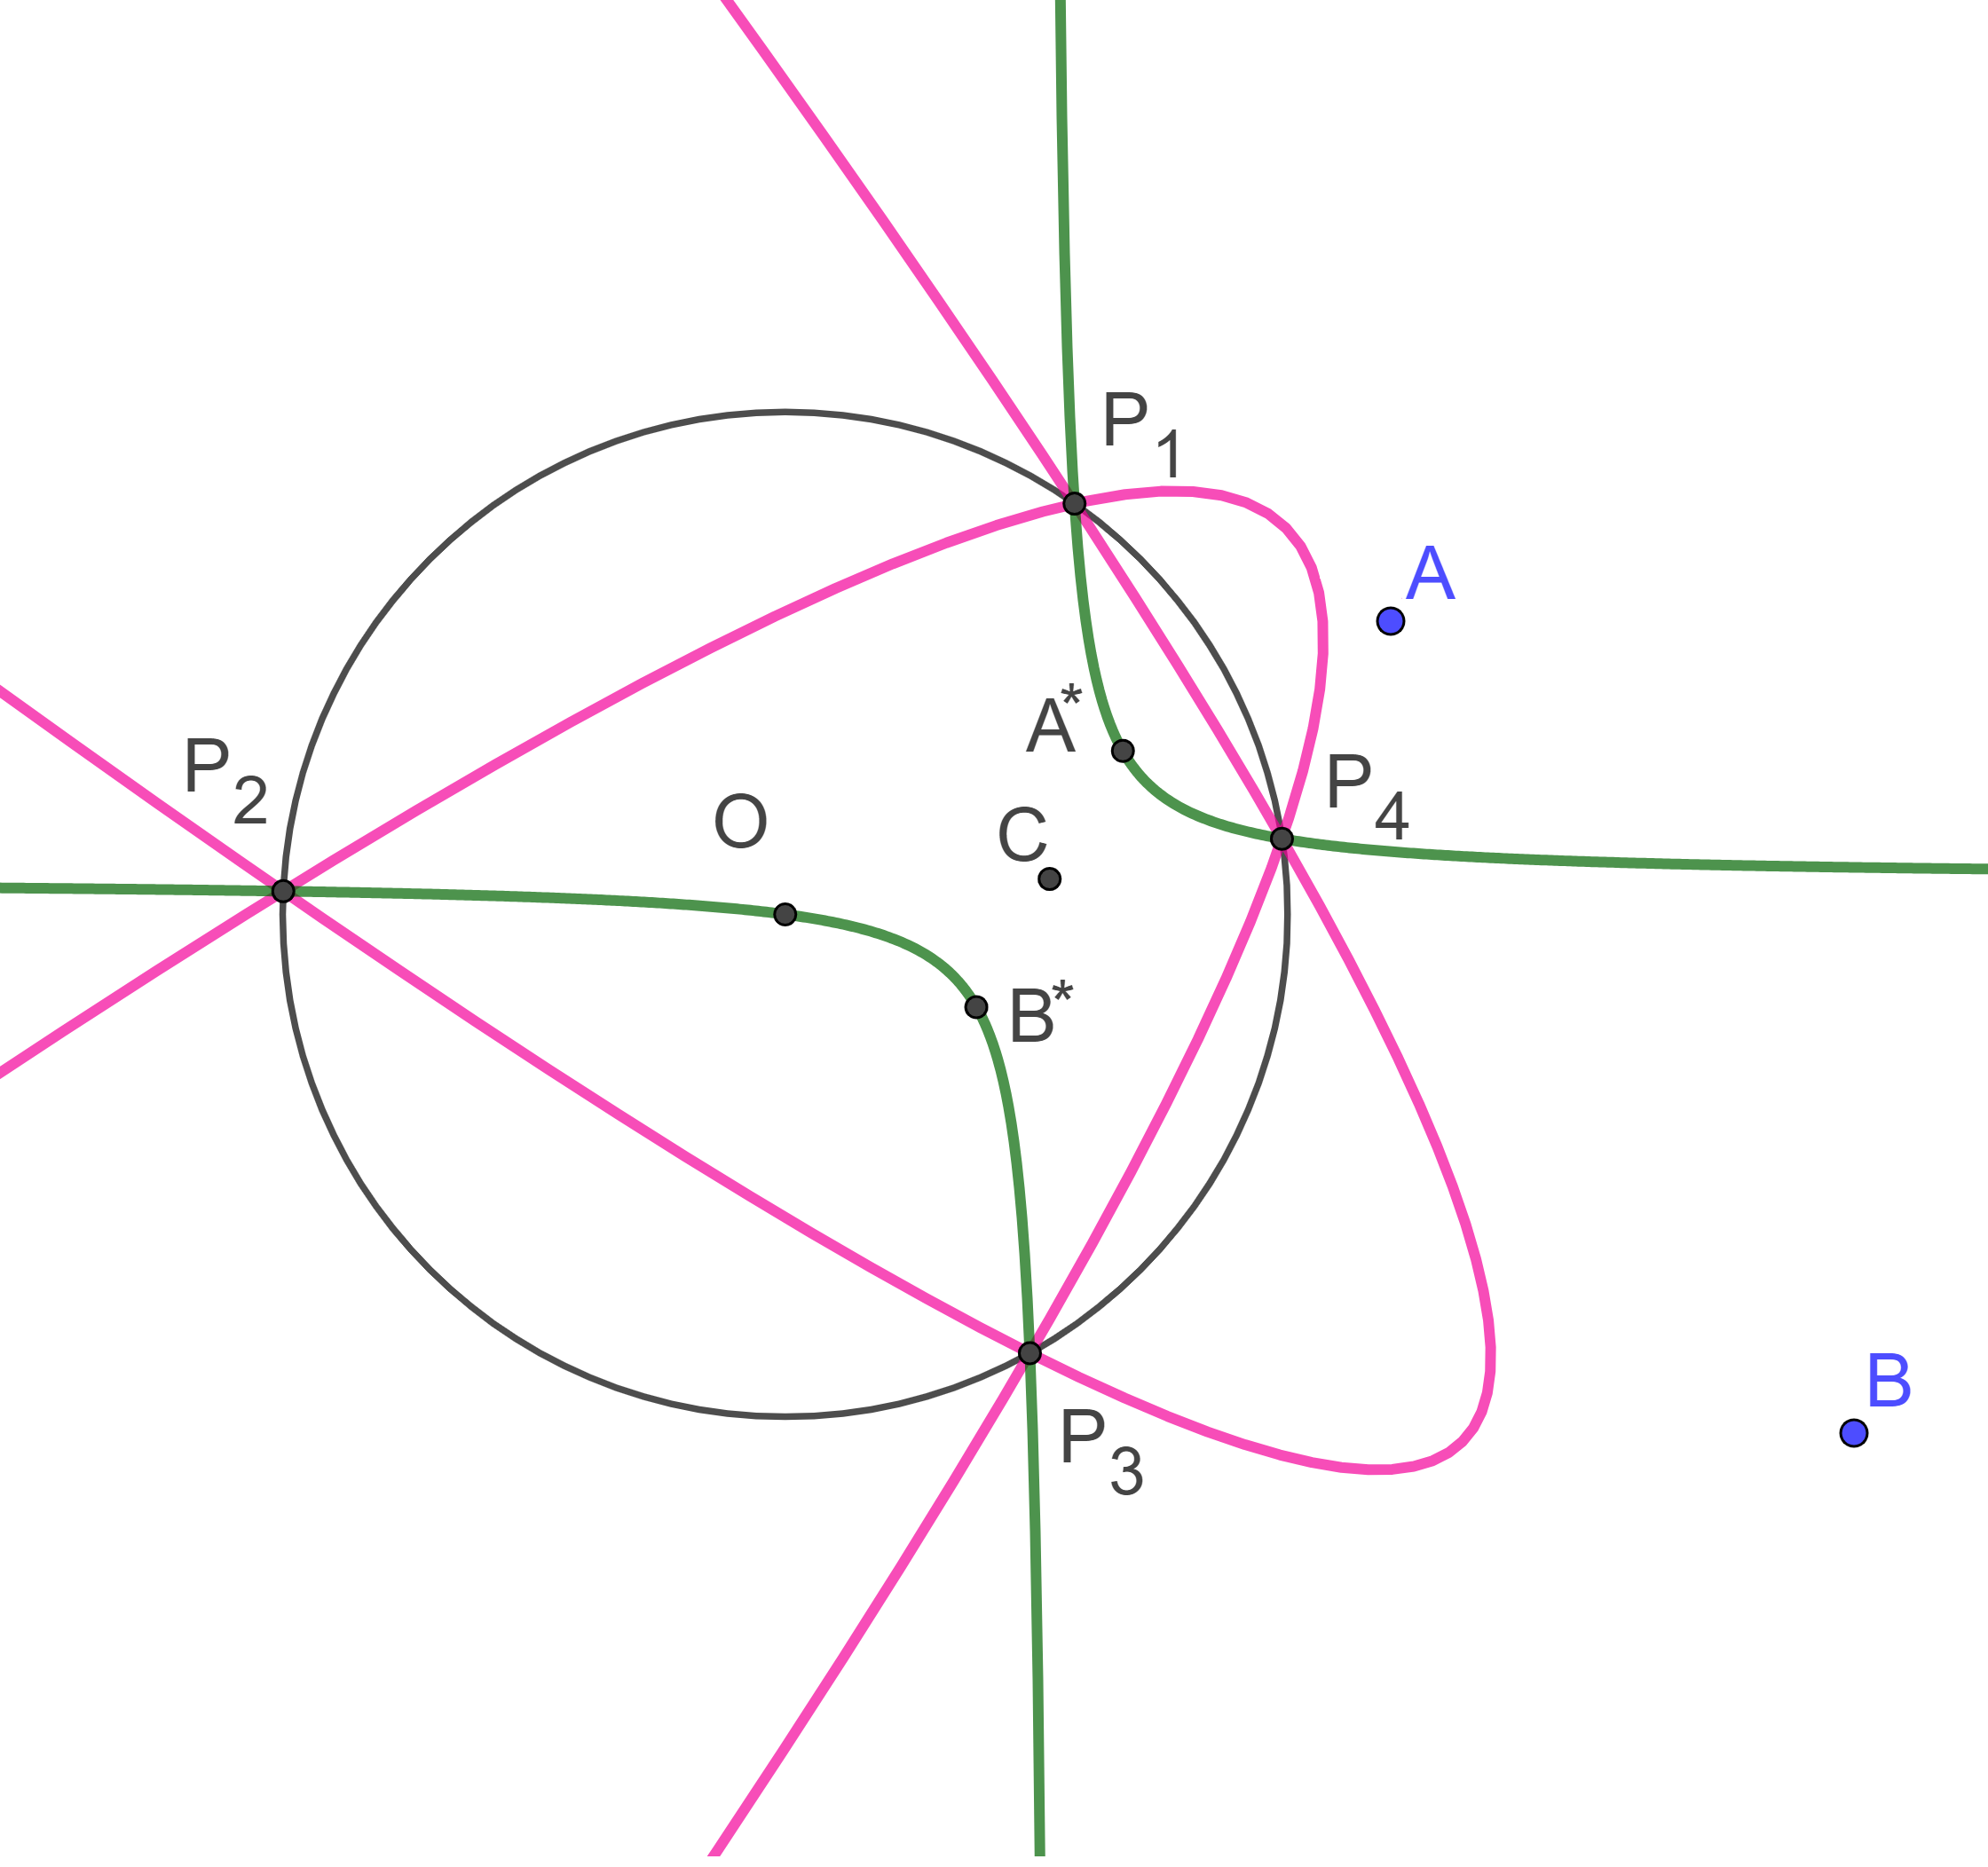
\includegraphics[width= 1\linewidth]{15}
		\caption{\small\textit{\color{lichsutoanhoc}Tìm nghiệm của bài toán bằng cách dựng hyperbola (màu xanh) hoặc parabola (màu hồng) rồi lấy giao điểm với đường tròn tâm $O$.}}
		\vspace*{-10pt}
	\end{figure}
	Các điểm ứng với các số phức $a^*$ và $b^*$ được định nghĩa ở phần trên là các điểm $A^*$ và $B^*$ trong hình. Ta có $O$, $A$ và $A^*$ thẳng hàng, $A$ và $A^*$ ở cùng phía so với $O$, và $OA^*\!\cdot\! OA\!=\!1$ (trong trường hợp bán kính đường tròn không bằng $1$ thì tích này bằng $R^2$). Tương tự với $B^*$. $A^*$ và $B^*$ còn gọi là ảnh của $A$ và $B$ qua vành phản xạ tròn. Do $c=\frac{a^* + b^*}{2}$ nên điểm $C(C_1,C_2)$ ứng với số phức $c$ chính là trung điểm của $A^*B^*$. Các tiệm cận của hyperbola song song với các trục tọa độ (một trục sẽ song song với phân giác của góc $AOB$, trục còn lại vuông góc với phân giác này). Một nhánh của hyperbola cũng sẽ đi qua điểm $O$. Cách dựng hyperbola này chính là lời giải mà Huygens đã tìm ra. Hyperbola này cũng chính là ảnh của đường cong Barrow qua mặt phản xạ tròn nên nó cũng đi qua cả $A^*$ và $B^*$.
	\vskip 0.1cm
	Nếu ta quay hệ trục tọa độ một góc $45^\circ$ ngược chiều kim đồng hồ thì tích $ab$ khi đó là một số ảo và phương trình mới của các số phức có dạng:
	\begin{align*}
		Z^2 + \overline{Z}^2 = 2(CZ + \overline{C}\overline{Z})
	\end{align*}
	với các chữ in hoa là tọa độ sau khi quay.
	\vskip 0.1cm
	Do đó:
	\begin{align*}
		X^2 - Y^2 = 2(C_1X - C_2Y)
	\end{align*}
	Tìm giao điểm của đường cong này với đường tròn $X^2+Y^2=1$, ta được hai parabola với các trục chính vuông góc nhau tại trung điểm của $OC$:
	\begin{align*}
		C_1X + \left(Y- \frac{1}{2}C_2^2\right)^2 &= \frac{1}{4}\left(C_2^2 + 2\right)\\
		\text{và } \left(X- \frac{1}{2}C_1^2\right) + C_2Y &= \frac{1}{4}\left(C_1^2 + 2\right).
	\end{align*}
	Các parabola này chính là lời giải của Sluse. Trục chính của chúng cắt nhau tại trung điểm của $OC$.
	\vskip 0.1cm
	Trong một số trường hợp, lời giải của ta sẽ suy biến.  Khi $A$, $O$ và $B$ thẳng hàng hoặc $AO = BO$ thì hai nhánh hyperbola sẽ biến thành hai đường thẳng $x=c_1$ và $y=0$. Đường cong Barrow trở thành hình gồm đường thẳng $y=0$ và một đường tròn đi qua $O$. Trong trường hợp $AO = BO$, đường tròn này đi qua $A$ và $B$.
	\begin{figure}[H]
		\vspace*{-5pt}
		\centering
		\captionsetup{labelformat= empty, justification=centering}
		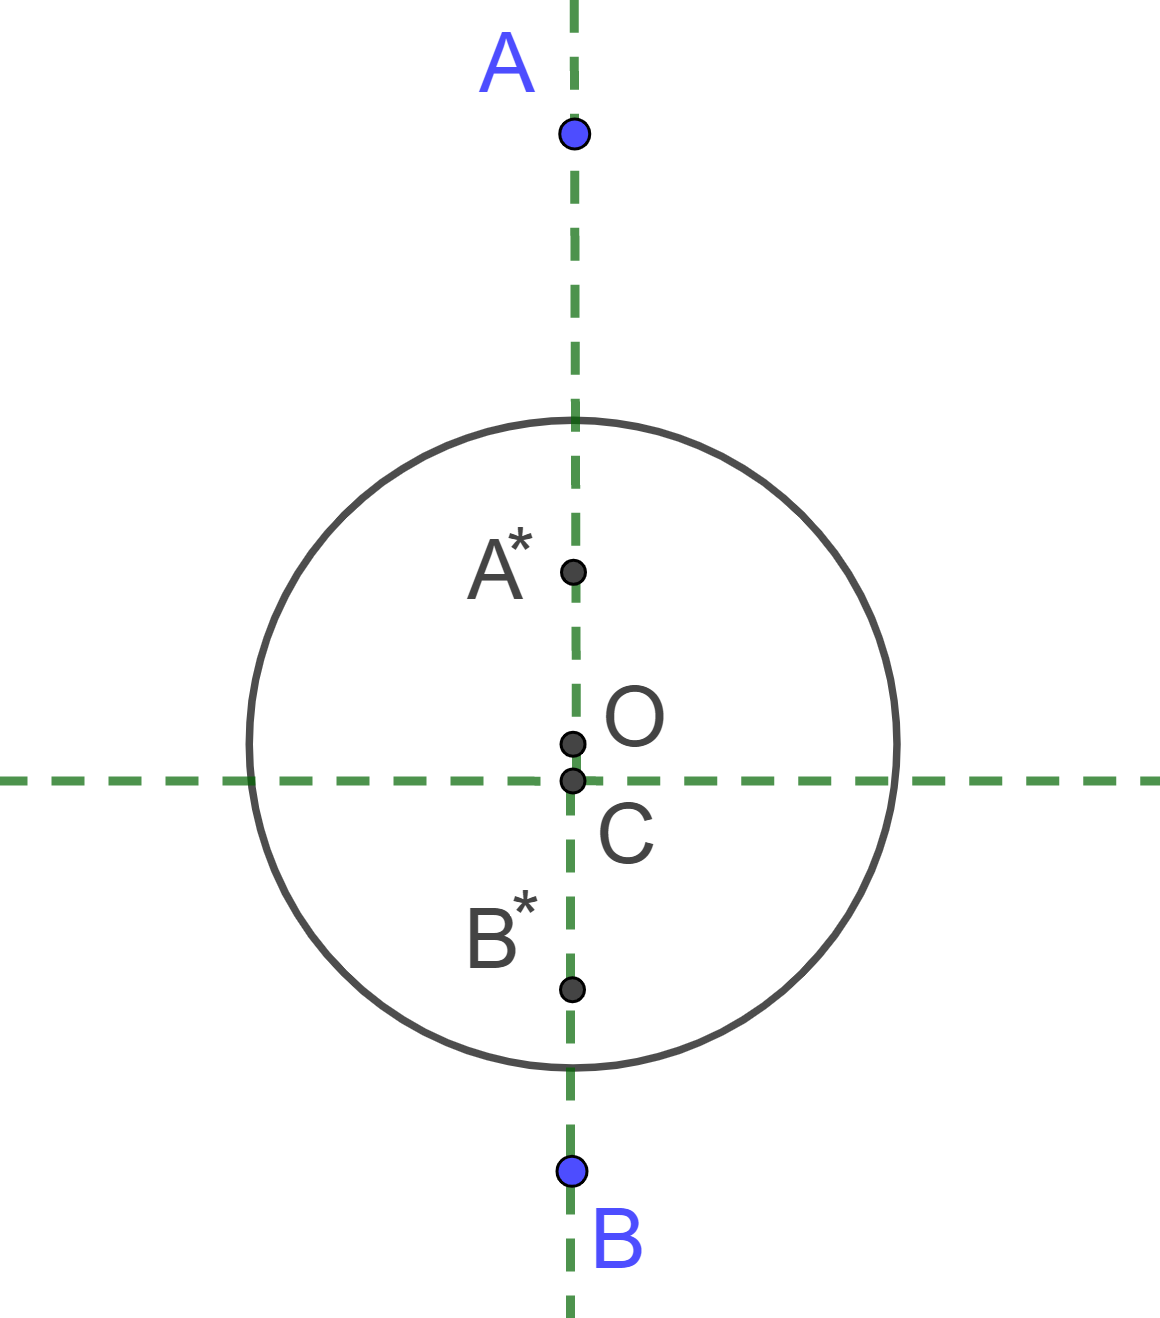
\includegraphics[width= 0.75\linewidth]{16}
		\caption{\small\textit{\color{lichsutoanhoc}Trường hợp $A$, $O$, $B$ thẳng hàng.}}
		\vspace*{-10pt}
	\end{figure}
	\begin{figure}[H]
		\vspace*{-5pt}
		\centering
		\captionsetup{labelformat= empty, justification=centering}
		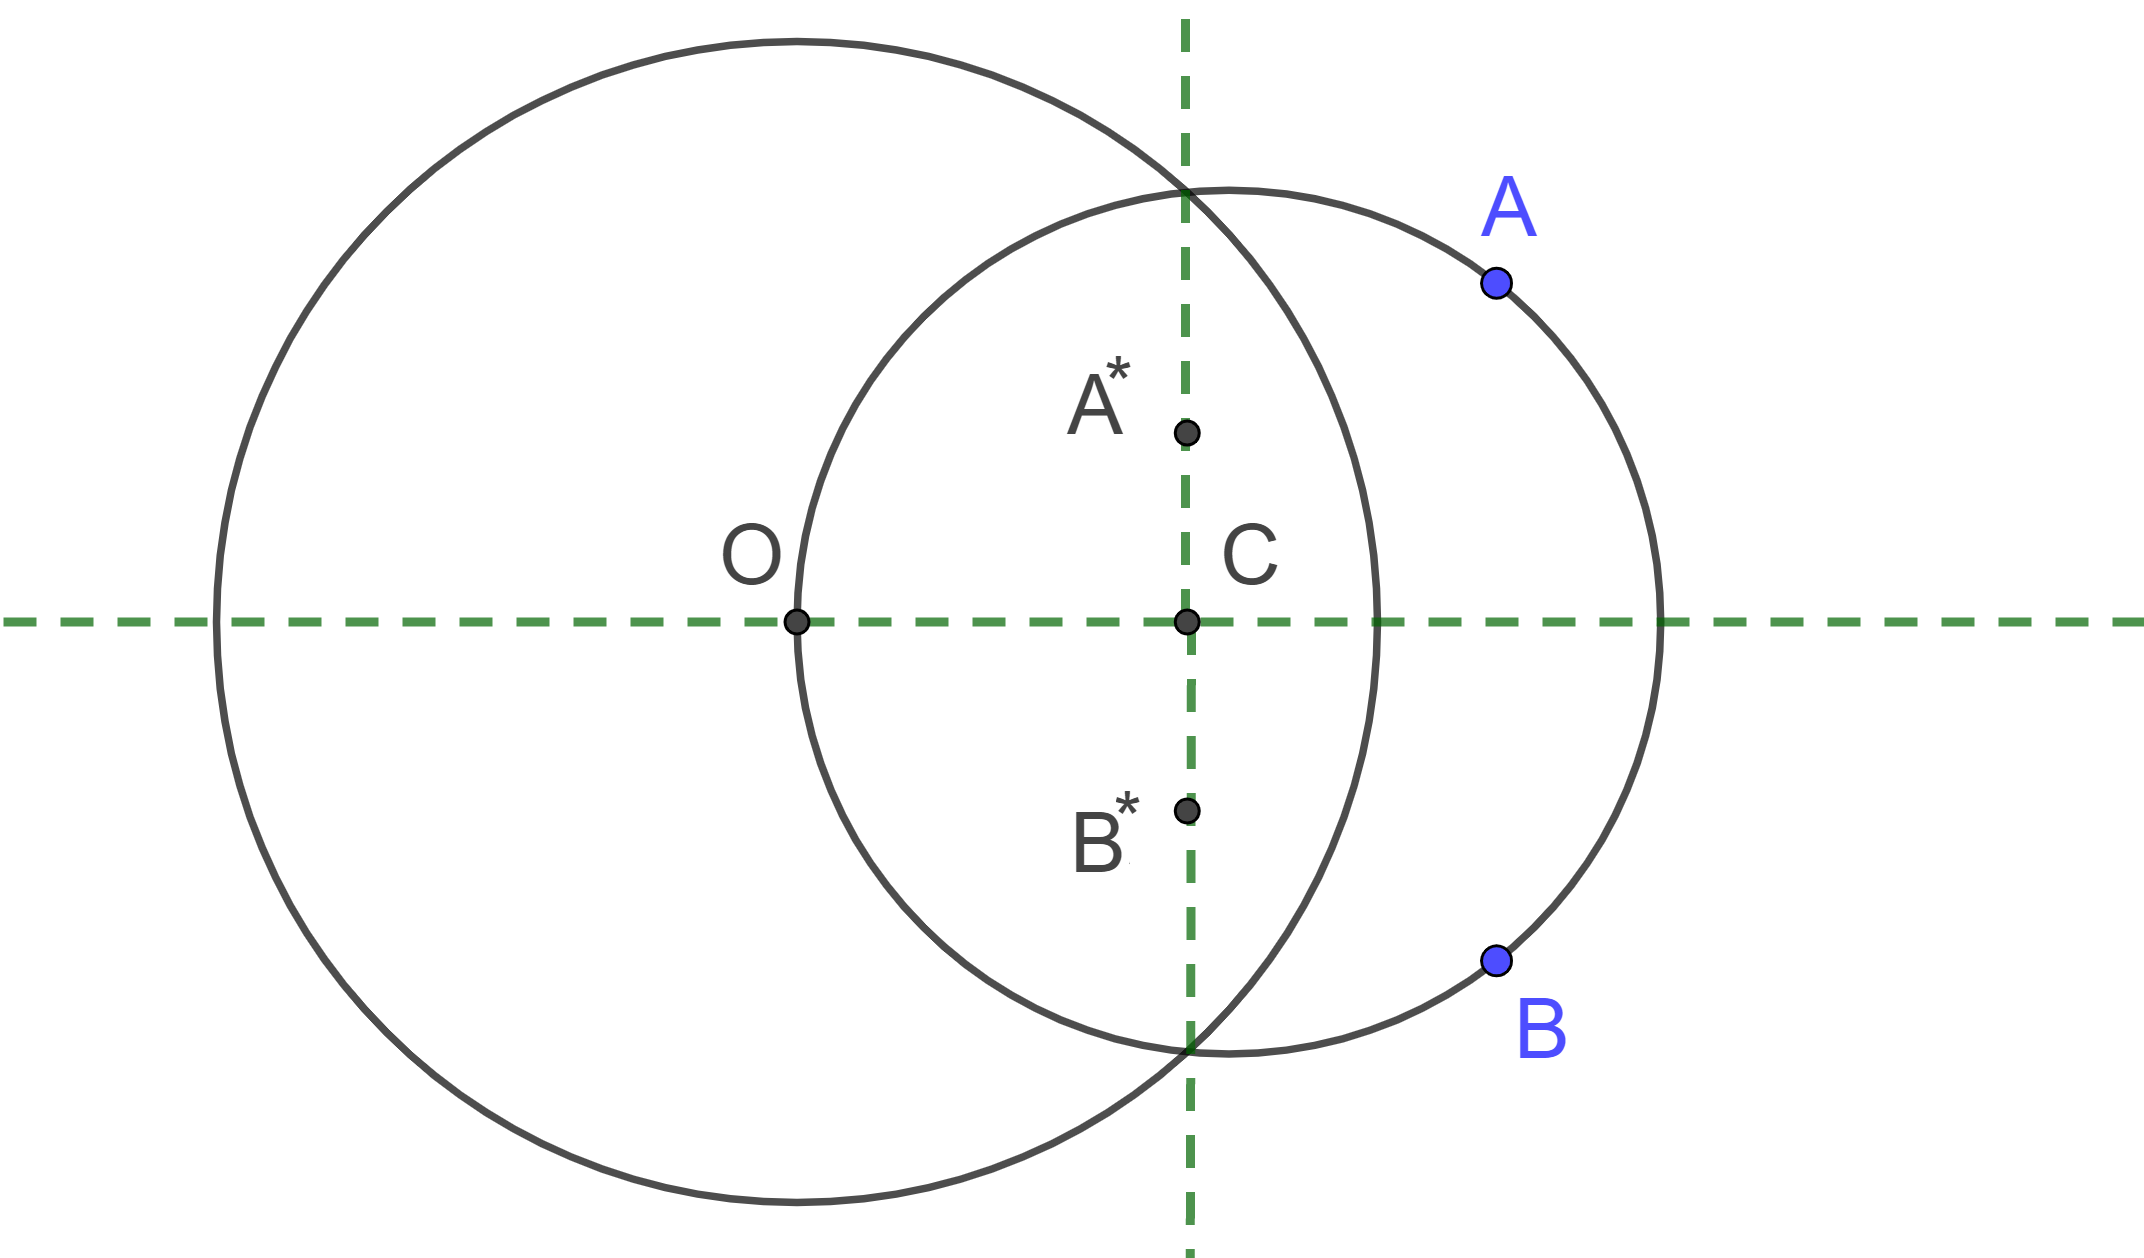
\includegraphics[width= 1\linewidth]{17}
		\caption{\small\textit{\color{lichsutoanhoc}Trường hợp $AO = BO$.}}
		\vspace*{-10pt}
	\end{figure}
	\textbf{\color{lichsutoanhoc}Bài tập}
	\vskip 0.1cm
	$1.$ Một bài toán khác của al--Haytham. Cho điểm $A$ nằm trong đường tròn tâm $O$. Tìm các điểm $B$ và $C$ trên đường tròn sao cho tia sáng từ $A$ đến $B$ phản xạ đến $C$ rồi quay về $A$. (Gợi ý: Đặt $OA = c$, $OB = OC = r$. Gọi $x$ là khoảng cách từ $O$ đến $BC$. Hãy chứng minh: $2cx^2+r^2x=cr^2$).
	\begin{figure}[H]
		\vspace*{-5pt}
		\centering
		\captionsetup{labelformat= empty, justification=centering}
		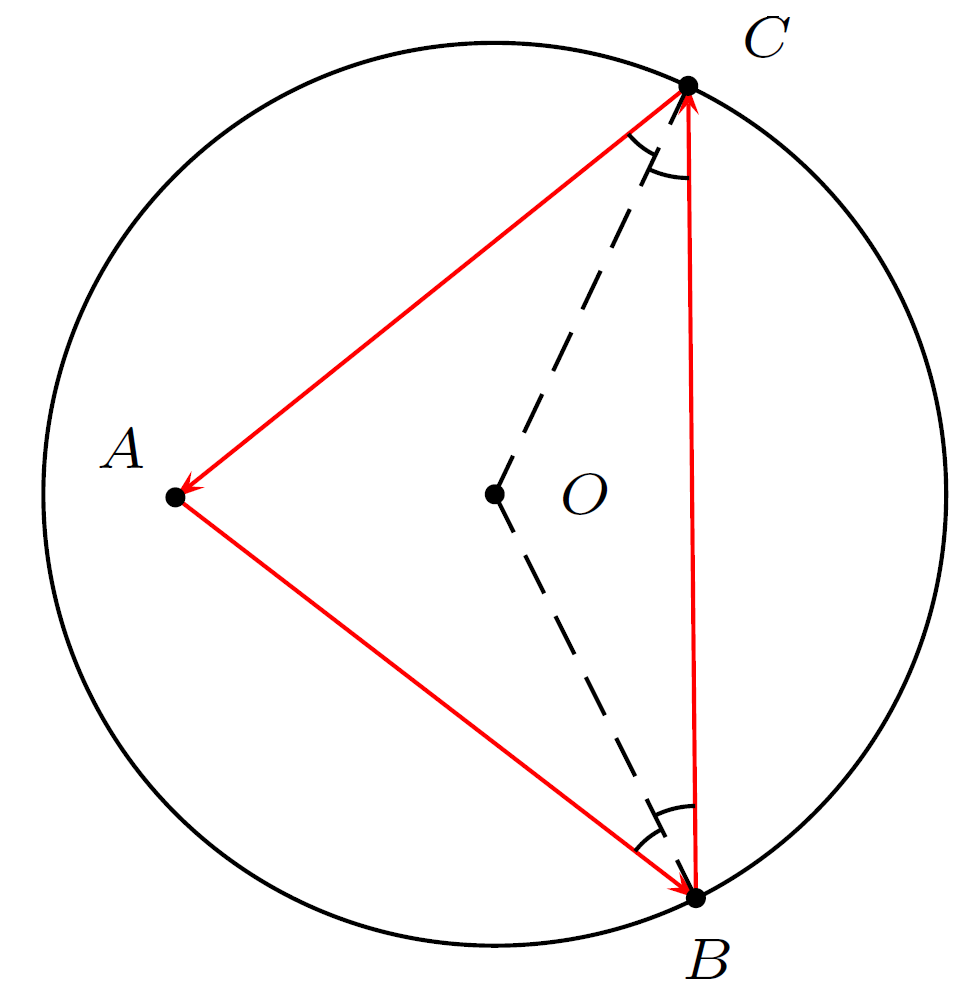
\includegraphics[width= 0.75\linewidth]{18}
		\vspace*{-10pt}
	\end{figure}
	\vskip 0.1cm
	\textbf{\color{lichsutoanhoc}Tài liệu tham khảo}
	\vskip 0.1cm
	[$1$] Drexler, M. and Gander, M.J. ($1998$). Circular Billiard. \textit{SIAM Review}, $40(2)$, pp.$315-323$. doi:$10.1137$/s$00361445963$\\$10872$.
	\vskip 0.1cm
	[$2$] Smith, J.D. ($1992$). The remarkable Ibn al--Haytham. \textit{The Mathematical Gazette}, [online] $76(475)$, pp.$189-198$. doi:$10.2307$/$3620392$.
	\vskip 0.1cm
	[$3$] Wilk, S.R. ($2015$). Ibn al--Haytham: $1000$ Years after the Kitāb al--Manāẓir. \textit{Optics and Photonics News}, $26(10)$, p.$42$. doi:$10.1364$/opn.$26.10.000042$.
	\vskip 0.1cm
	[$4$] Winter, H.J.J. ($1953$). THE OPTICAL RESEARCHES OF IBN AL--HAITHAM. Centaurus, $3(1)$, pp.$190-210$. doi:$10.1111$\\/j.$1600-0498$.$1953$.tb$00529$.x.
\end{multicols}